\documentclass[english,ngerman,parskip=half]{scrartcl}
\usepackage{amsmath}
\usepackage{amssymb}
\usepackage{amsthm}
%\usepackage[portuges]{babel}
\usepackage[utf8]{inputenc}
\usepackage{graphicx}
\usepackage[T1]{fontenc}
\usepackage{systeme}
\newcommand{\abs}[1]{\lvert #1 \rvert}

%\usepackage{libertine}
\usepackage{microtype}
\usepackage{lmodern}
\usepackage[brazilian]{babel}
\usepackage{xcolor}


\begin{document}
 %capa copiada de https://tex.stackexchange.com/questions/177283/create-a-cover-for-my-thesis
 %start Cover

    \begin{titlepage}
        \vspace*{-3cm}
        %\makebox[\dimexpr\textwidth+2cm][r]{\includegraphics[height=1.5cm]{FULogoRGB(1)}} 
        \makebox[\dimexpr\textwidth+2cm][r]{
\includegraphics[height=1.5cm]{./images/marca-udesc.png}} 

        \vspace*{5cm}
    \begin{center}
        \Huge\bfseries\sffamily Jogos Psicomotores

        \vspace*{2cm}
        \large 
        Formulário de Jogo Materiais Didático-Pedagógicos
        para o Ensino de Matemática
    \end{center}

    \enlargethispage{3cm}
    \vfill
    \parbox[t]{0.45\textwidth}{%
            %Matrikelnummer: 1234572              \\
                Área: Matemática \\
                    Universidade: UDESC/CCT \\
                    {\selectlanguage{brazilian}\today}
                          }%
                          \hfill
                          \begin{tabular}[t]{l@{}}%{\raggedleft%
                              Professora:\\
                                Dr. Tatiana Comiotto
                              \end{tabular}
                              %}%
                          \end{titlepage}
% end Cover

\begin{itemize}

    \item \textbf{Nome:} Bingo dos polinômios
    \item \textbf{Colaboradores:} \\
        Bruno da Silva Esmeraldino
        \\
        Mateus Schroeder da Silva
    \item \textbf{Conteúdos abordados:}
        \begin{itemize}
            \item Operações com polinômios (Multiplicação);
            \item Valor numérico de um polinômio.
            \item Trabalhar a concentração, a capacidade de análise/síntese e o raciocínio dos participantes.
        \end{itemize}
    \item \textbf{Objetivo:}
        \begin{itemize} 
            \item Operações com polinômios (Multiplicação);
            \item Valor numérico de um polinômio.
            \item Trabalhar a concentração, a capacidade de análise/síntese e o raciocínio dos participantes.
        \end{itemize} 
    \item \textbf{Regras/como aplicar:} 
            \begin{itemize}
                \item O jogo pode ser jogando por no máximo 4 pessoas. 
                \item Para jogar, lançam-se sobre a mesa os  dados e efetua-se a operação de multiplicação correspondente.
                \item Uma vez escolhida a ordem e efetuado o cálculo de forma correta, o aluno deve colocar um de seus pinos no tabuleiro correspondente à expressão correta do resultado.
                \item Se alguém conseguir preencher três casas consecutivas, na horizontal,vertical ou diagonal, vencerá o jogo. 
            \end{itemize}

        \begin{figure}[ht!]
            \centering
            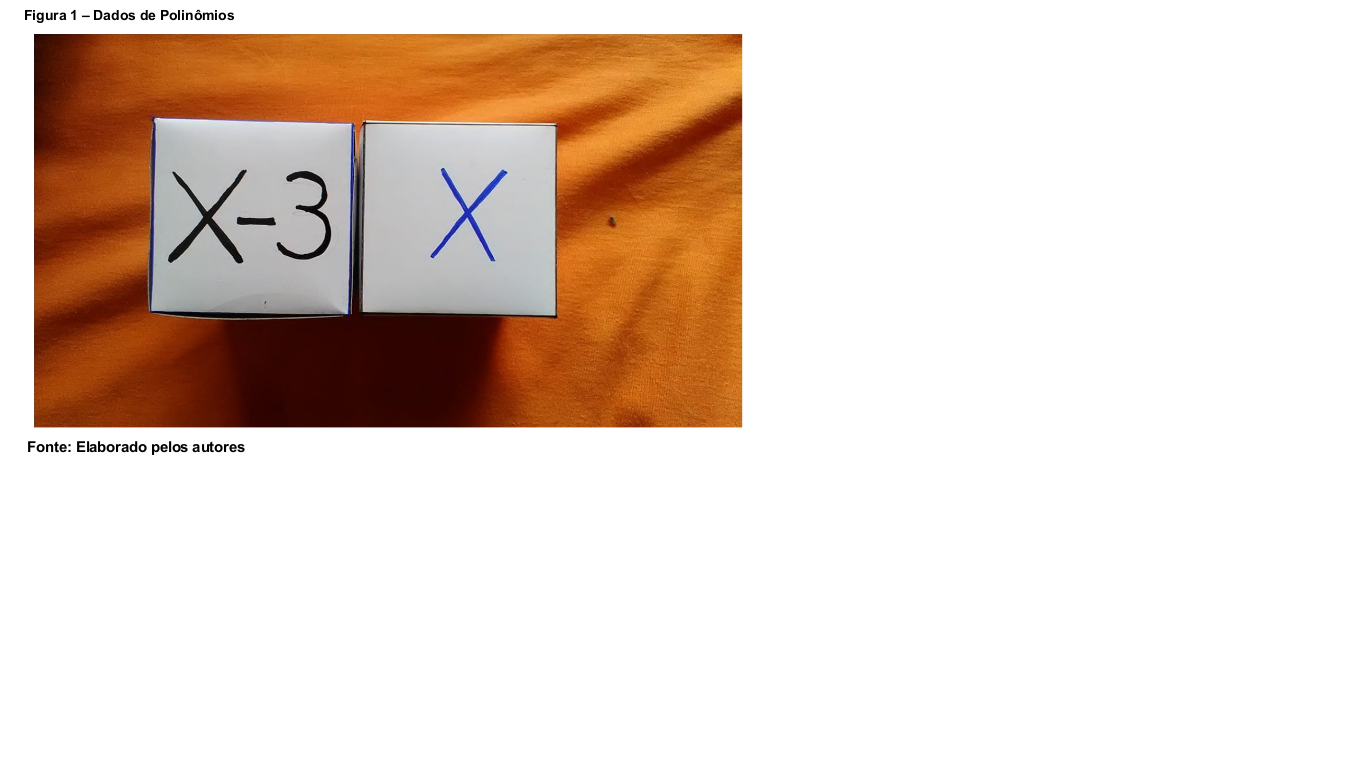
\includegraphics[width=90mm]{./images/dados.png}
            \caption{Dados\label{Dados}}
        \end{figure}

        \begin{figure}[ht!]
            \centering
            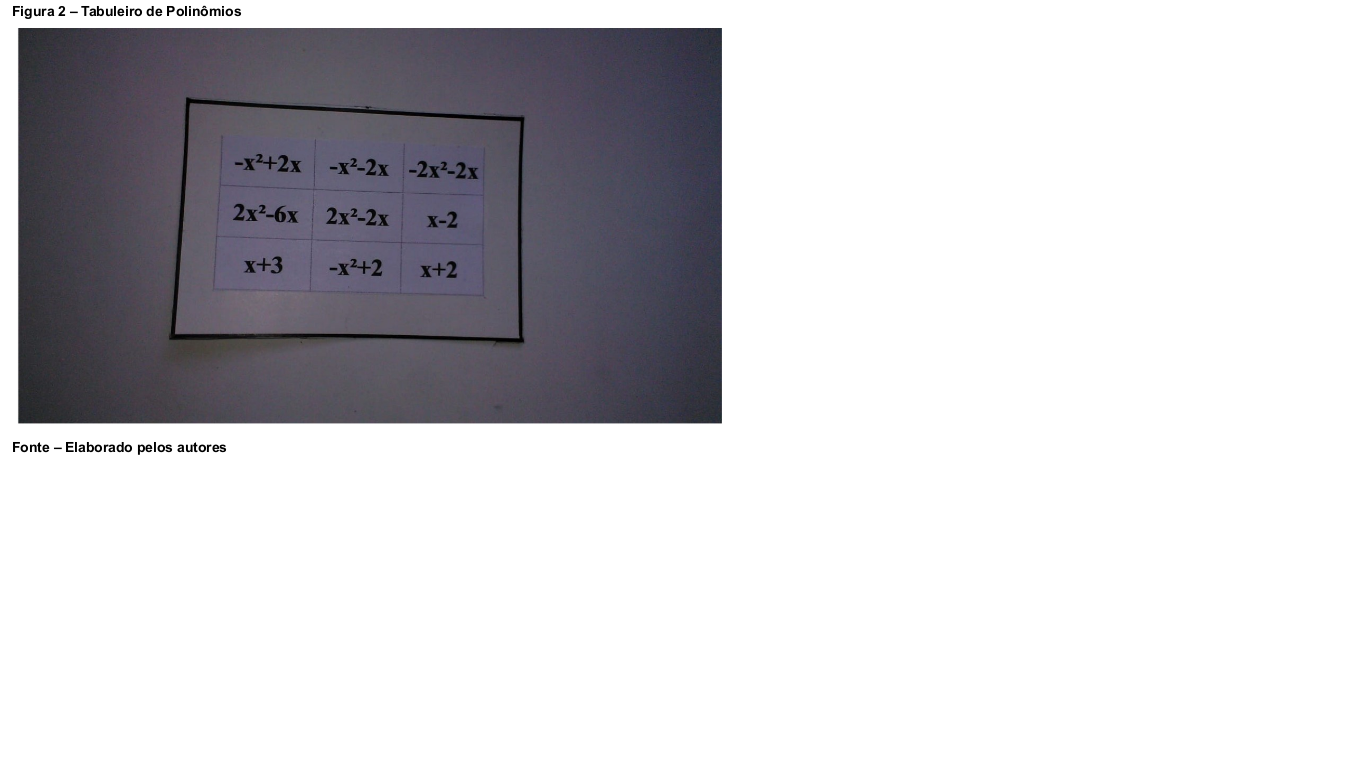
\includegraphics[width=90mm]{./images/cartela.png}
            \caption{Cartela\label{Cartela}}
        \end{figure}

        \begin{figure}[ht!]
            \centering
            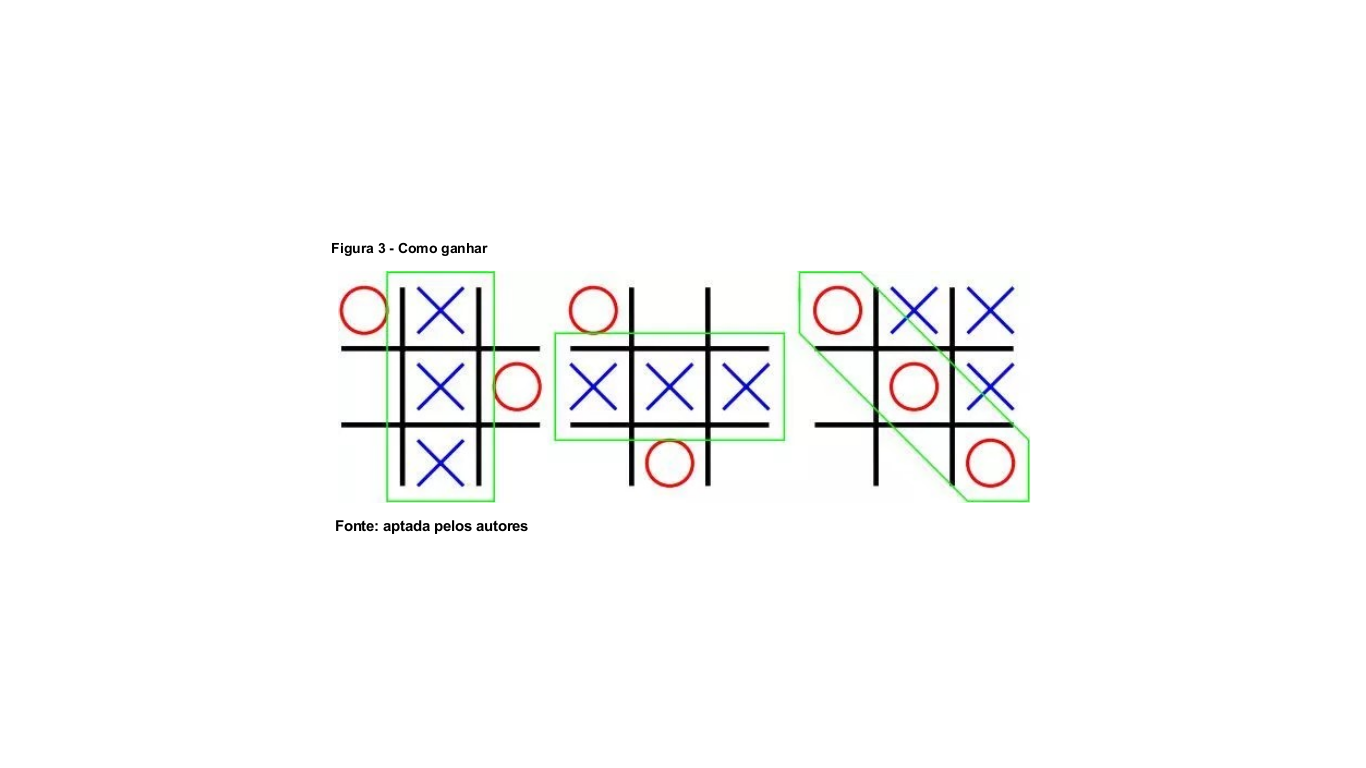
\includegraphics[width=90mm]{./images/crit-vit.png}
            \caption{Critérios de vitória\label{Critérios de vitória}}
        \end{figure}

\end{itemize}
\newpage
\begin{itemize}

    \item \textbf{Nome:} Quebra-cabeça triangular
    \item \textbf{Colaboradores:}\\
        Bruno da Silva Esmeraldino
        \\
        Mateus Schroeder da Silva
    \item \textbf{Conteúdos abordados:} Expressões algébricas, produtos notáveis e operações elementares.
    \item \textbf{Objetivo:} Servir como uma maneira diferente de fazer exercícios sobre o assunto de polinômios e das operações elementares.
    \item \textbf{Regras/como aplicar:} 
            \begin{itemize}
                \item O jogo termina quando um triângulo maior contendo todas os triângulos menores for formado, respeitando que os lados dos triângulos menores (de lado 1) tem de cada lado expressões de mesmo valor.
                \item De 1-5 jogadores.
            \end{itemize}

        \begin{figure}[ht!]
            \centering
            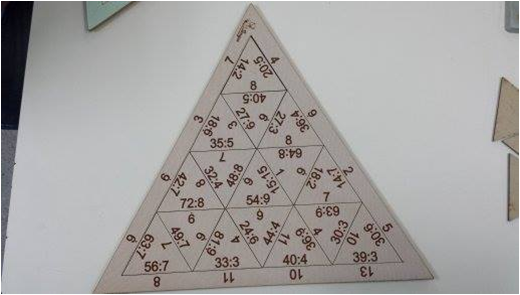
\includegraphics[width=90mm]{./images/qc-comprado.png}
            \caption{Quebra-cabeça de divisão (base)\label{Quebra-cabeça de divisão}}
        \end{figure}

        \begin{figure}[ht!]
            \centering
            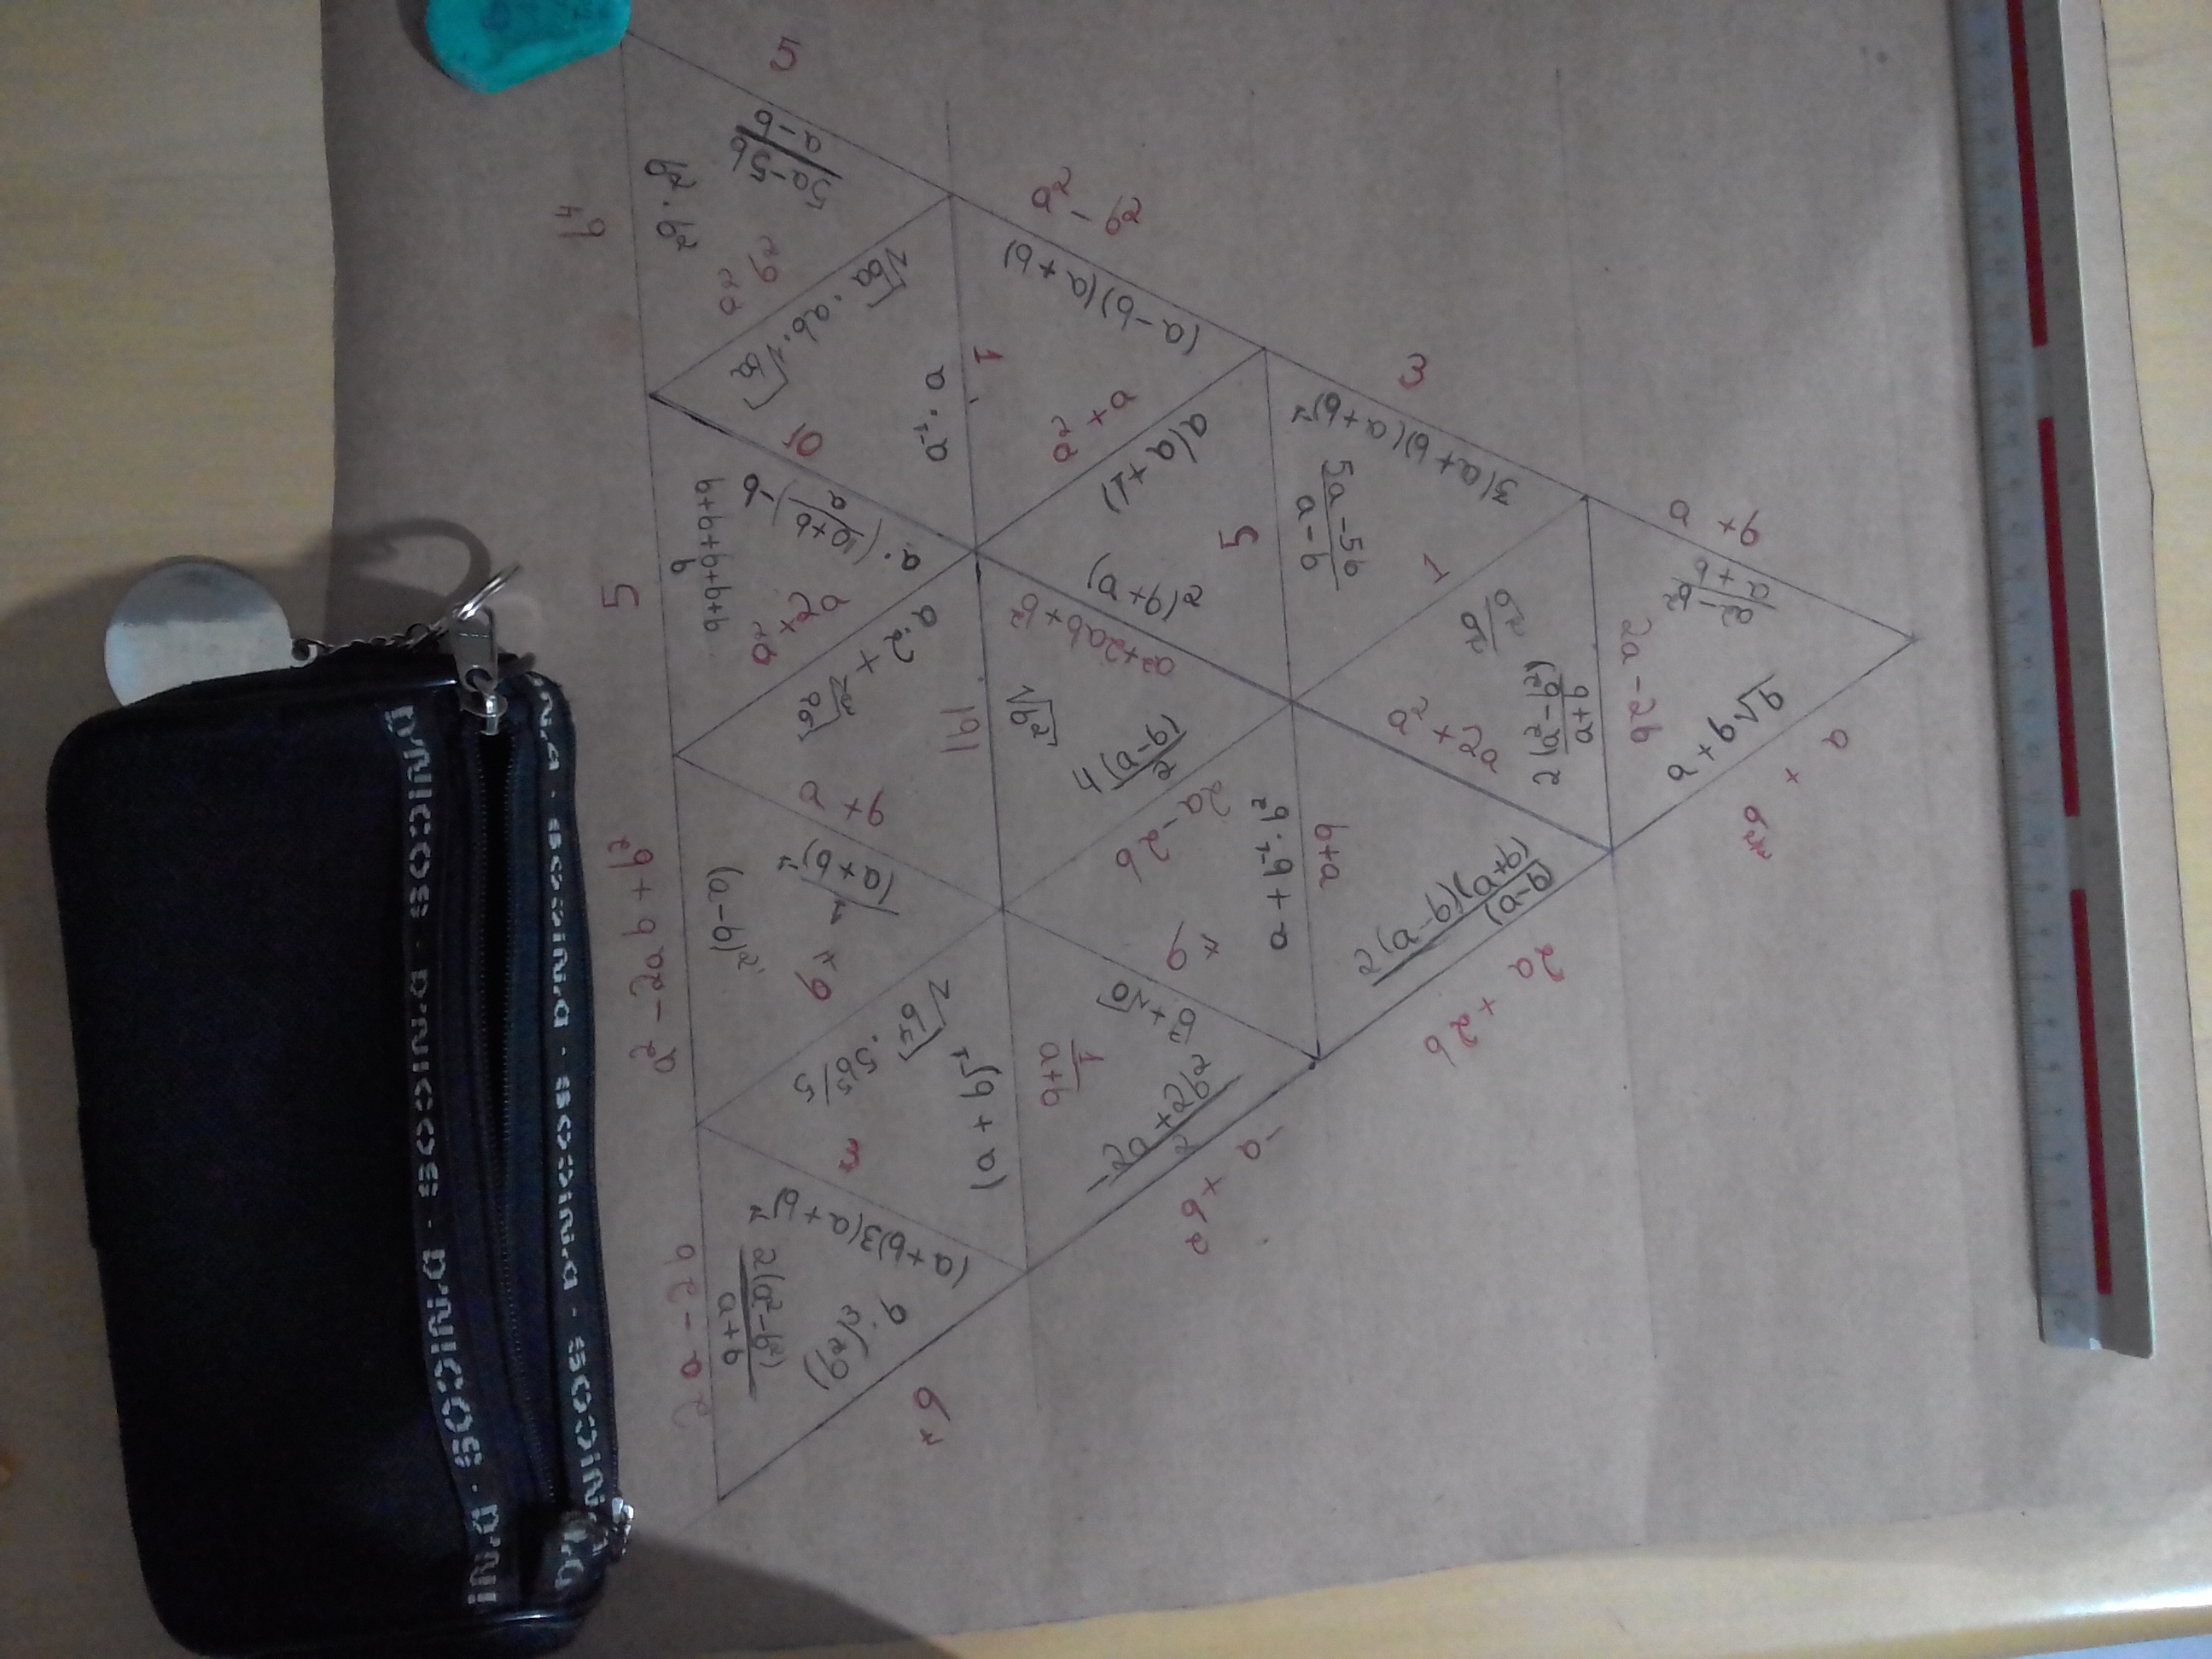
\includegraphics[width=90mm]{./images/qc-polinomial.jpg}
            \caption{Quebra-cabeça de polinômios e expressões algébricas\label{Quebra-cabeça de 'polinômios'}}
        \end{figure}

\end{itemize}
\end{document}

